\subsection{Commercial Use}
Over the last decade, we have seen huge advancements in commercial devices such as cellular devices, computers, and gaming consoles. Providing users an alternative form of interaction can allow all groups. Google is currently developing an experimental project named 'Soli' that uses radar-detected gestures for touch-free gesture controls.
public-ally available devices such as the Google Pixel have implemented this technology at the top of the smartphone. Soli is supported in applications such as Google Music for skipping tracks and Pokemon wave rendering wave gestures and responding with a wave back from the Pokemon on screen.


  
  \begin{figure}[h!]
  \centering
    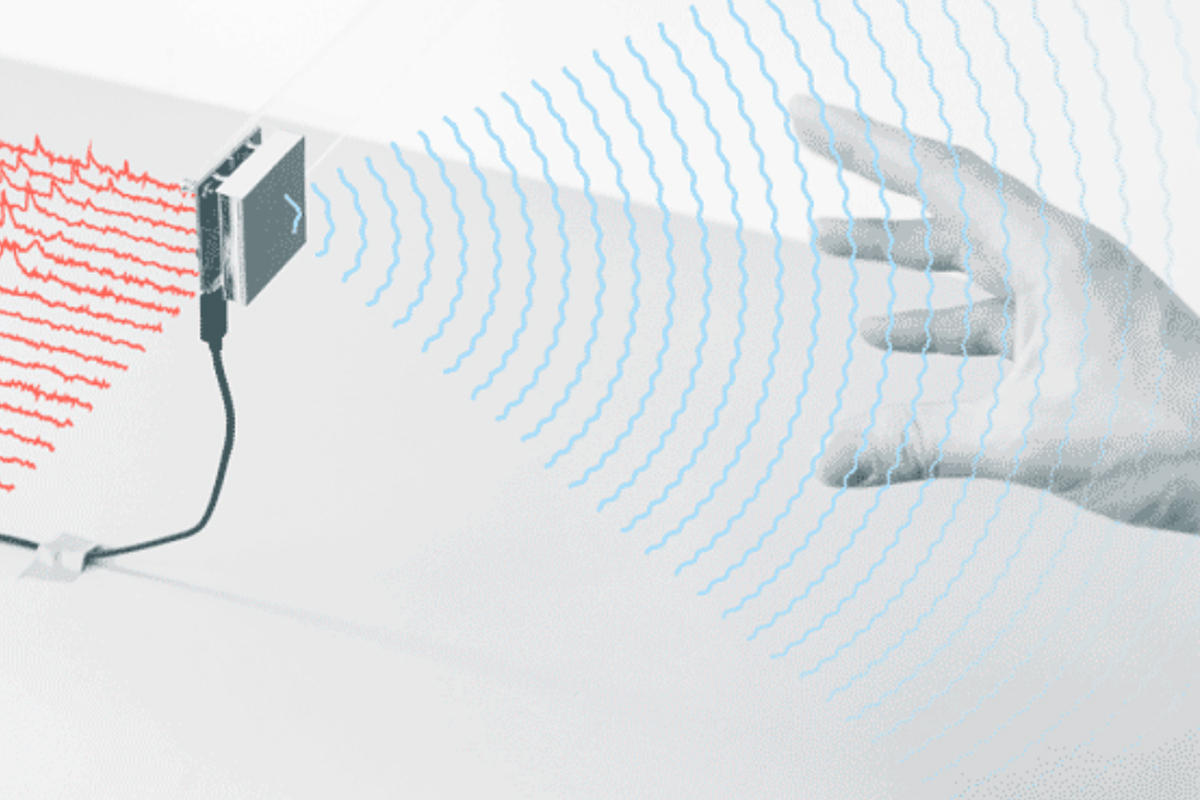
\includegraphics[width=0.7\textwidth]{Research-Latex/images/GoogleRadar.jpg}
     \caption{Googles Project  Soli}
\end{figure}
  
\subsection{Requirements for use }

Gestures are developed around the basis of the human who is trying to interact with the computer holding the gesture recognition system. Humans have been researching gesture systems as early as the 1980s.The human must know the language the machine is operating by for example 'hand pal' the computer must have the gesture mapped and displayed by the machine. It is required for the computer two have three entry points 
\begin{enumerate}
  \item (Software:)There must be a software project with the appropriate software using machine learning or any subset of artificial intelligence. A prime example of gesture recognition is Microsoft's Cortana.
  \item (Hardware:)There must be a piece of hardware in place for the camera sensor to capture users' movement.
\item (User: ) The end user being behind the computer with a knowledge of the basic gestures for the programs features.

\end{enumerate}




\subsection{Disabilities}
A huge benefit of the implementation of gesture-based user interfaces is allowing individuals with mental and or physical disabilities to interact with devices which usually inoperable. People with physical conditions such as Parkinson's cannot interact with traditional hardware such as keyboards and computer mouses. Currently, three students from the Royal College of Art have developed a recognition system for amputees by way of two white, silicone discs containing inertial measurement unit sensors. A startup company named Limix are currently developing gesture recognition to record Deaf peoples hand movement and translate into words and read via an assistant voice reader.

 \begin{figure}[h!]
  \centering
    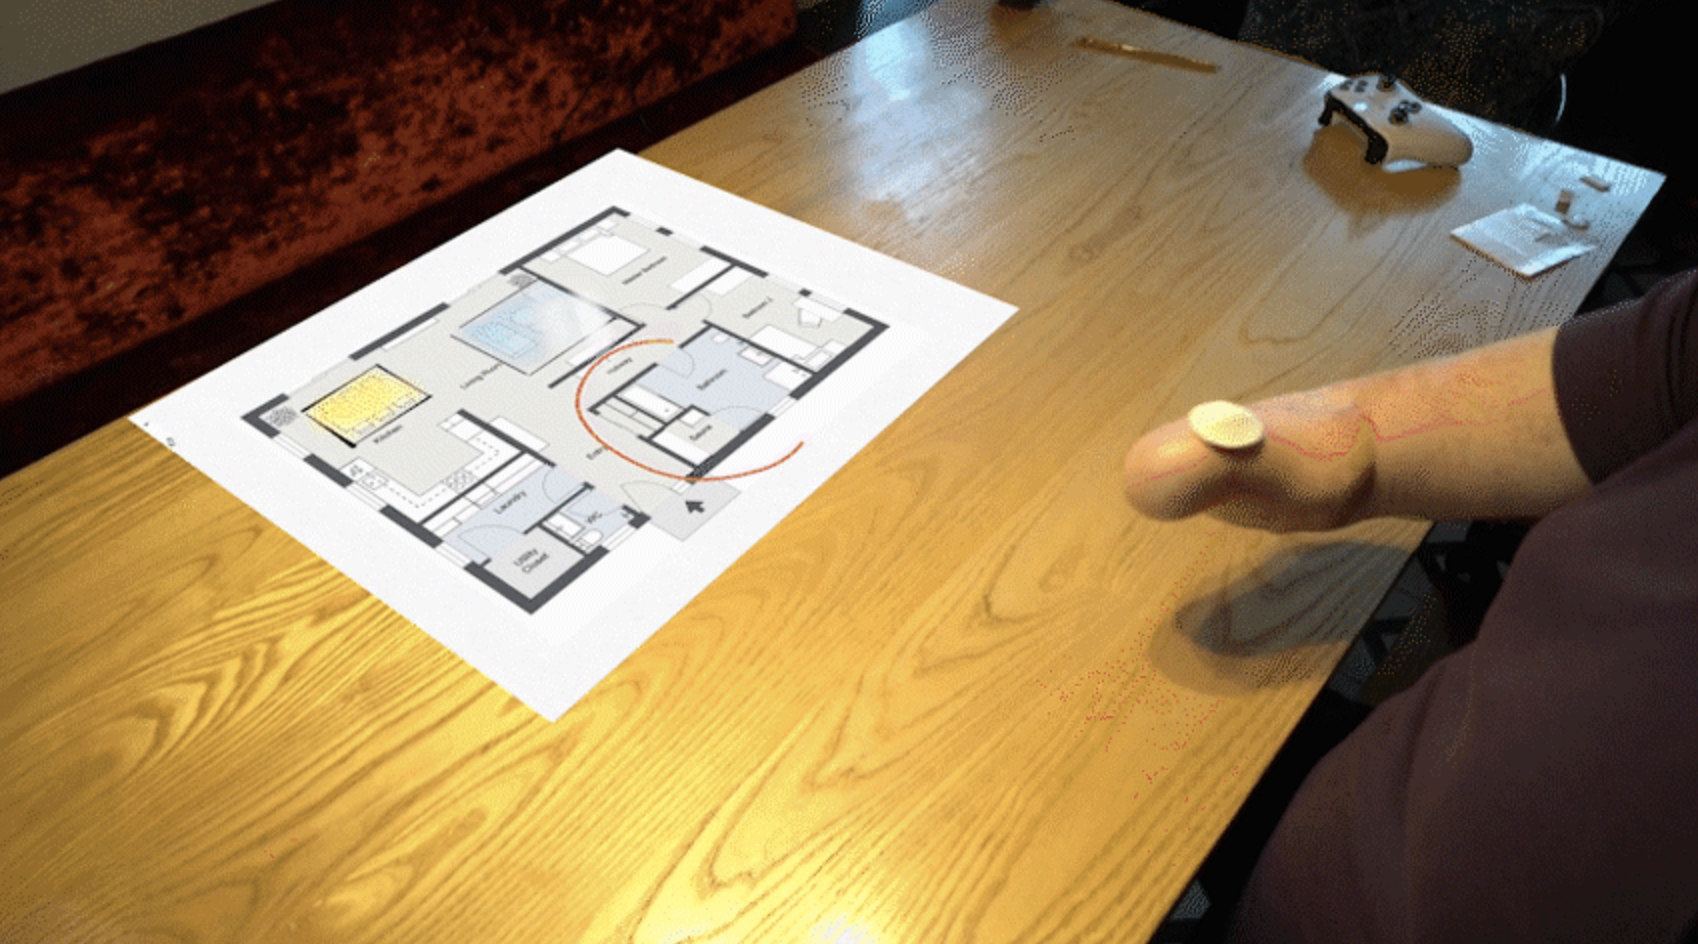
\includegraphics[width=0.7\textwidth]{Research-Latex/images/PeopleWithDisabilities.png}
     \caption{Two dots motion sensors allowing drawing gesture}
\end{figure}
 


Italian start-up Limix uses gesture recognition named ' Talking Hands' to record the sign language hand movements of deaf people while wearing glove-like hardware. They are then translated into words, which are played by a voice synthesizer on a smartphone. The product is still in the development phase will be a breakthrough for gesture systems and for communication tools for people with disabilities.




   \begin{figure}[h!]
  \centering
    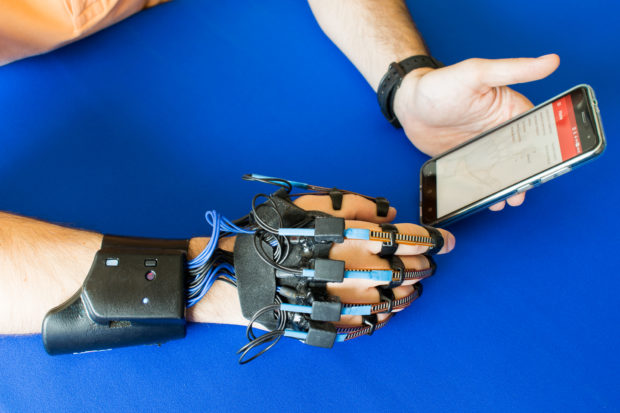
\includegraphics[width=0.5\textwidth]{Research-Latex/images/talkingHandsPrototype.jpg}
     \caption{Talking Hands Wearable tech Prototype to track deaf peoples hand movement}
\end{figure}
 